\documentclass[10pt, a4paper]{article}
\usepackage{lrec2016}
\usepackage{multibib}
\newcites{languageresource}{Language Resources}
\usepackage{graphicx}
% for eps graphics

\usepackage{epstopdf}
\usepackage[latin1]{inputenc}
 

\title{Open Source Code Serving Endangered Languages}

\name{Richard Littauer, Hugh Paterson III}




%
%         Saarbr\"ucken, Germany, Oregon, USA\\
%         richard.littauer@gmail.com, hugh_paterson@sil.org\\}


\address{Saarland University, SIL International\\
         Saarbr\"ucken, Germany, Oregon, USA\\%, Address2, Address3 \\
         richard.littauer@gmail.com, hugh\_paterson@sil.org\\}%, author2@zzz.edu, author3@hhh.com\\}


\abstract{
We present a database of open source code that can be used by low-resource language
communities to build digital resources. Our database is also useful to software developers
working with those communities and to researchers looking to describe the state of the field
when seeking funding for development projects.  \\ 
\newline 
\Keywords{open source, under-resourced languages, database, endangered languages, code, computational resources} }

\begin{document}

\maketitleabstract

\section{Introduction}

Almost half of the approximately 7,000 currently spoken languages are expected to
become extinct this century; it is estimated that less than 5\% of these will be used online or have significant digital presence \cite{kornai2013digital}. Languages which do not have significant digital resources (often called low-resource, under-resourced, or minority languages) risk extinction from loss of prestige, specific domain usage (such as online), and ultimately loss of speakers.

Many language communities and academics working with them try to prevent this by developing
tools, websites, and resources for their languages. However, these approaches are fragmented,
often incurring large developmental and funding costs for single, non-extensible use cases. 

To make this process easier for all stakeholders, we have built the first database (to our knowledge) of all open source code projects related to low-resource languages.

Our database is structured as a simple list (in Markdown format), hosted in a GitHub repository. GitHub is the largest online network of open source code and allows for parallel collaborative development, while providing critical collaborating support via a built in wiki, issue tracking and comments on new suggestions. The features provided by Github are increasingly important to academics and the field of education (Zagalsky 2015). These features were not available via previous code and text sharing solutions such as SourceForge and are often not available via institutional repositories. 

Our list is structurally simple, shareable, easily updated, and part of a wider cultural movement on GitHub of using Markdown files as simple databases (Sorhus 2013). Our list monopolizes on the low barrier of entry on GitHub (Storey et al. 2014). Because the list is part of GitHub, and because it is not maintained, funded, or dependent upon a large institution or funding body (but rather run by independent contributors), the list itself is a novel way of crowd-sourcing data and resources from the linguists, computational linguists, and coders who would use the tools themselves. 

Our list currently describes over 241 open source projects, which includes specific sections for extensible code for over 26 different languages.

Our solution is open source, not just in the sense of code and data availability (or disclosure) but
in the sense of collaborative involvement and inclusive discussion. By using a solution like
GitHub we were able to reach out to both developers and researchers. Our list is updatable more rapidly than previous solutions like http://lingtransoft.info/, or other resources like GOLD (http://linguistics-ontology.org/), ELCAT (http://www.endangeredlanguages.com/), or OLAC (http://www.language-archives.org/) . We mitigate the risk of a single point of failure (a recent issue with LinguistList) by working in a distributed fashion. The data in our list is open and can be copied and reused by anyone, something not necessarily true of previous solutions. By choosing such a solution, we sidestep many of the institution issues associated with archives and repositories currently servicing academics.

Our ultimate goal is a collaboratively built and maintained resource for highlighting
useful, extensible code for low-resource languages. We would like to share our current efforts
and welcome communication with the wider academic linguistics community.

\section{Database structure}

The list itself largely consists is a single Markdown file. This is useful for a couple of reasons; first, there's no need for a gateway or endpoint to access the content of the database, as there would be if it were coded in SQL, RDF, or some other relational database. Secondly, people can search the list using their browser and the standard search feature for any website. Finally, the list can be digested immediately instead of depending on searches to get complete coverage of the data. 

\subsubsection{Categories}

Within the list, there are several main sections where we attempt to categorize the resources, based on user input and upon the best guesses of the maintainers about the functionality of the various tools. These sections are: Generic repositories (which includes massive dictionary and lexicography projects, single language lexicography projects, utilities, presentations of data, and software), i18n-related repositories, audio automation, text-automation, experimentation, flashcards, natural language generation, computing systems, android applications, Chrome extensions, FieldDB, FieldDB web-services and components and plugins, academic research paper-specific repositories, example repositories, and language  and code interfaces. 

We also have two other lists: One of other open source linguistic organisations, on GitHub, and other OSS (Open Source software) organisations, and another for language-specific projects, which includes subsections for code which is relevant to: Amharic, Arabic, Bengali, Chichewa, Estonian, Georgian, Guarani, Hausa, Hindi, H�gnorsk, Inuktitut, Irish, Japanese, Kinyarwanda, Korean, Lingala, Malay, Malagasy, Migmaq, Minderico, Nishnaabe, Oromo, Quechua, Sami, Scottish Gaelic, Secwepemcts�n, Somali, Tigrinya, Zulu.

Finally, we also include a short list of closed source resources which can still be utilized for free. 

\subsubsection{Example entry}

Each entry is a single line, containing the name of the resource, a link to the resource, and a short description. If the resource is also a GitHub repository, we include a link to a badge that shows the amount of stars (similar to likes or favorites on other social media sites, and, generally, a good proxy for usage and developer uptake of the resource) for that repository.

Here is one such entry: "* [Chichewa ![GitHub stars ](https://img.shields.io/github/stars/kscanne/chichewa.svg) ](https://github.com/kscanne/chichewa)  NLP resources for Chichewa"

\section{Personas and Stakeholders}

The list that we are maintaining is not aimed at any one group in isolation. Instead, there are several key groups whom we think may derive value from this list. These are as follows: Project Managers, Software Developers, Community Developers, and  Linguists, 

\subsection{Project Managers}

Project managers are generally linguists or community members who have been tasked with developing language resources, but generally don't have the skill to understand the technical aspects on their own (and thus are different from software developers). Many project managers do not have strong information technology project management backgrounds. However, they are often skilled linguists who have access to grant funding. The finer details of carrying out a project in a manner which benefits more than one language community is simply out of scope for many first time managers, and projects. We hope that project managers should be able to look at our list to be able to determine two things: 1. Has the project task, goals, or relevant deliverables already been accomplished for another language (or indeed, for the same language), and 2. where can they find the code base for that project so that they can integrate it into their own workflow. We hope, as well, that some project managers might be able to have a project used case and that they can use our list to answer the question of how to get funding for their idea. 

\subsection{Software Developers}

Software developers are often looking to find pre-existing solutions, and to find pre-existing modules which can be applied to new use cases they are asked to solve. Every problem which has already been solved by someone else is time that does not have to be spent developing. Every major project today uses open source code in some capacity, partially for this reason. This is in some ways the opposite perspective from the project manager, who are looking to develop something new and may not be looking for extensible solutions to their problem. The developer is looking for use cases to which they can apply or reapply their code. We hope that our list makes this easy. 

One developer, at least, has said that this was the case: "Thanks a lot for pointing me to the list. It is awesome! It has some really good tools and resources which would be very useful in a lot of things that I am doing. I shall definitely add some of my resources and tools to this list....I have also come across a very useful library - Poio-api - on your list which is a parser for most of these XML files that I work with." (Personal communication, 2015)

\subsection{Community Developers doing Language Development}

This may include language development organizations, or individuals who are "community members" looking to deploy their own solutions. They want to know ?does it work with my language? by which they often, but not always mean ?written language?. An additional complexity, is that there are different perspectives on what ?does it work? really mean. The degree of technologicalization in the majority culture affects the expectation of the kinds of real world tasks desired to be accomplished in the low-resourced language. Tasks might be sending SMS messages in a particular script. But sometimes, users of low-resource languages have a very different expectation and interaction with technology. For instance, members of deaf communities require video integration in their digital solutions more than many other kinds of Low-resource languages, but deaf communities may still need other tools commonly shared with written languages - like dictionary tools.

\subsection{Linguists}

We define linguists here as researchers who are not tech savy, but who are working in academia or directly with language communities from an academic perspective. Linguists, as such, are generally looking for patterns in language data. They want tools which are going to be easy to use to find the patterns they are looking for and present the data in ways which help others to understand the purpose and meaning of those patterns. As end users, they are more likely to be looking for tools which are useful out of the box, and so may not be able to appreciate all of the items in the list, but still may benefit from a quick search through it. 
As well, we provide many links to tools that can be used with ELAN (http://www.mpi.nl/corpus/html/elan/), Praat (http://www.fon.hum.uva.nl/praat/), and other audio software which are used on a day-to-day basis by many linguists themselves. 

\section{Commitments}

Unlike most projects, which must depend upon institutions, private or public funding, or volunteers, this project has no single point of failure. The list itself is currently hosted by Richard Littauer's GitHub account, but due to the nature of a Git repository and of collaborative work on GitHub, any replication of the list can be edited, stand alone, and be used if the original project goes down for any reason. The decentralized quality of git repositories makes this list a much less brittle solution than database or institutional repositories. 

As well, there is a very low possibility of misuse; if any one person using the program decides to enforce their own viewpoint, perspective, or rules at the cost of any other user group or of the community, it is entirely possible for anyone else to make a copy of the list and to then use that as the source of truth going forward. 

One possible issue with the list is that if a malicious user takes over the main list. Then, it would take some time for any other list to have the same clout in the community. This is, however, true of all existing databases. A good example, although not open data, is the Ethnologue, which recently added a paywall to their database about languages (but not to the ISO 639-3 standard which SIL International also stewards). The loss of a previously costlessly accessible resource became a major source of contention for many linguists, although SIL International had legitimate reasons for doing so (namely, the financial cost of hosting the database). 

One of the future goals of the project is to develop a community where anyone can ask questions about the list and its resources, and other users can help out and give advice easily. While this is possible with GitHub issues, it depends upon a higher amount of usage of the list itself than currently exists. Marketing the list in tech conferences is one possible solution. 

\section{Conclusion}

We have here outlined our reasons for developing a list of open source software for endangered languages. We hope that this resource is used by the community, and that this paper fosters discussion and awareness of open source resources. 

%TODO: Add the references in 
%% References
%-1. Endangered Languages. https://www.github.com/RichardLitt/endangered-languages
%-2 Kornai A (2013) Digital Language Death. PLoS ONE 8(10): e77056. doi:10.1371/journal.pone.0077056
%-3 GitHub. https://www.github.com
%-4 SourceForge. https://www.sourceforge.com
%-5 Sindre Sorhus?s list of awesome-lists. https://github.com/sindresorhus/awesome
%6. Lingtransoft. http://lingtransoft.info/
%7. Linguist List. 


% Past reviewer statements

% Reviewer 1:
% The abstract states the problem well - namely, that languages with few resources need more computational support.

% The main point seems to be that the author has collected a list of other people's work. However, I find it impossible to determine whether the author's work supports the main point due to the lack of examples or even a basic description of the project's structure. It does not seem innovative in that it does not seek to present a new method for providing resources, only a new way of collecting existing methods.

% If the work is as described, it is relevant to the field and may have a significant impact on applied linguistic material & resource creation for less-served language communities. It's just very difficult to assess it without sufficient evidence.
% Reviewer 2:

% The authors present an interesting project, well suited for a poster or digital poster presentation, but not for an oral presentation.
% Many participants at the LSA would benefit from learning about this project and vice versa the authors would find additional resources among the participants.
% Reviewer 3:

% This is a presentation of a tool rather than a research paper. Maybe include results from testing for particular languages.
% Reviewer 4:

% This paper is valuable as it mitigates a basic problem in the field of language documentation, extending a potential wealth of resources to those who would traditionally have higher barriers to them.

% There are a few basic questions that ought to be addressed: 

% It is clear that this project is intended at linguists. Would good to develop or pitch in such a way that it can be useful to community members (who may not have the resource of a linguist)?

% What are the stakeholders' commitments to this project? Bearing in mind that it serves under-resourced communities that will always exist, it will be good to hear how such a project may exist for a good duration.

% Because this is open-source, are there guidelines in place for the misuse of available code and projects?

% Is there a central community that will be able to advise users who face difficulties when using the system?

% I would recommend this as a paper rather than a poster, seeing that this brings valuable a new valuable tool to the field. It might not be as effective in poster form.


%
%\section{Citing References in the Text}
%
%\subsection{Bibliographical References}
%
%All bibliographical references within the text should be placed in parentheses
%containing the author's surname followed by a comma before the date of
%publication \cite{Martin-90}. If the sentence already includes the author's
%name, then it is only necessary to put the date in parentheses:
%\newcite{Martin-90}. When several authors are cited, those references should be
%separated with a semicolon: \cite{Martin-90,CastorPollux-92}. When the reference
%has more than three authors, only cite the name of the first author followed by
%et al. (e.g. \cite{Superman-Batman-Catwoman-Spiderman-00}).
%%
%\subsection{Language Resource References}
%
%\subsubsection{When Citing Language Resources}
%
%When mentioning language resources, we recommend that they are cited in
%a similar way to bibliographical references, except that, in order to make them
%appear in a separate section, you need to use the
%\texttt{\\citelanguageresource} tag. Thus, a language resource should be cited
%as \citelanguageresource{speecon}.
%
%
%\subsubsection{When Not Citing Any Language Resource}
%
%When no language resource needs to be cited in the paper, you need to comment
%out a few lines in the \texttt{.tex} file:
%
%\begin{verbatim}
%% \usepackage{multibib}
%% \newcites{languageresource}{}
%% \section{Language Resource References}
%% \bibliographystylelanguageresource
%%   {lrec2016}
%% \bibliographylanguageresource{xample}
%\end{verbatim}
%
%\section{Figures \& Tables}
%\subsection{Figures}
%
%All figures should be centred and clearly distinguishable. They should never be
%drawn by hand, and the lines must be very dark in order to ensure a high-quality
%printed version. Figures should be numbered in the text, and have a caption in
%Times 10 pt underneath. A space must be left between each figure and its
%respective caption. 
%
%Example of a figure enclosed in a box:
%
%\begin{figure}[!h]
%\begin{center}
%%\fbox{\parbox{6cm}{
%%This is a figure with a caption.}}
%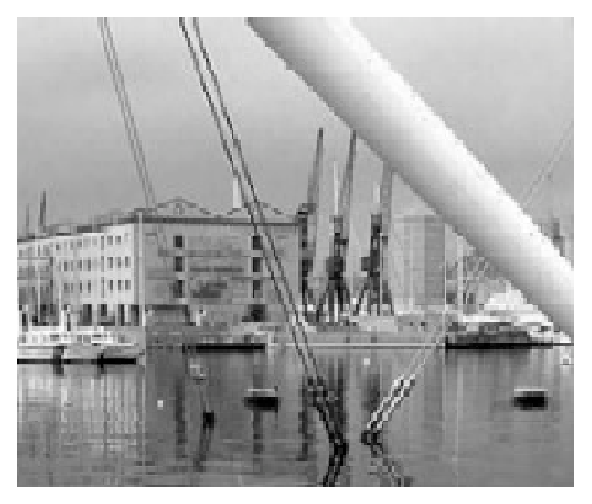
\includegraphics[scale=0.5]{image1.eps} 
%\caption{The caption of the figure.}
%\label{fig.1}
%\end{center}
%\end{figure}
%
%Figure and caption should always appear together on the same page. Large figures
%can be centred, using a full page.
%%NB: an example of large figures is missing.  \newpage
%
%\subsection{Tables}
%
%The instructions for tables are the same as for figures.
%%Two types of tables are distinguished: in-column and big tables that don't fit in the columns.
%%\subsection{In-column tables}
%%An example of an in-column table is presented here.
%%
%\begin{table}[!h]
%\begin{center}
%\begin{tabular}{|l|l|}
%
%      \hline
%      Level&Tools\\
%      \hline\hline
%      Morphology & Pitrat Analyser\\
%      Syntax & LFG Analyser (C-Structure)\\
%     % Semantics & LFG F-Structures + Sowa's\\
%     % & Conceptual Graphs\\
%      \hline
%
%\end{tabular}
%\caption{The caption of the table}
% \end{center}
%\end{table}
%
%%\subsection{Big tables}
%%
%%An example of a big table which extends beyond the column and will
%%float in the next page.
%%
%% \begin{table*}[ht]
%% \begin{center}
%% \begin{tabular}{|l|l|}
%%
%%       \hline
%%       Level&Tools\\
%%       \hline\hline
%%       Morphology & Pitrat Analyser\\
%%       Syntax & LFG Analyser (C-Structure)\\
%%       Semantics & LFG F-Structures + Sowa's Conceptual Graphs  \\
%%       \hline
%%
%% \end{tabular}
%% \caption{The caption of the big table}
%% \end{center}
%% \end{table*}
%%
%
%\section{Footnotes}
%
%Footnotes are indicated within the text by a number in superscript\footnote{They
%should be in Times 9, and appear at the bottom of the same page as their
%corresponding number. Footnotes should also be separated from the rest of the
%text by a horizontal line 5 cm long.}.
%
%\section{Copyrights}
%
%The The Lan\-gua\-ge Re\-sour\-ce and Evalua\-tion Con\-fe\-rence (LREC)
%proceedings are published by the European Language Resources Association (ELRA).
%They are available online from the conference website.
%
%
%ELRA's policy is to acquire copyright for all LREC contributions. In assigning
%your copyright, you are not forfeiting your right to use your contribution
%elsewhere. This you may do without seeking permission and is subject only to
%normal acknowledgement to the LREC proceedings. The LREC 2016 Proceedings are
%licensed under CC-BY-NC, the Creative Commons Attribution-NonCommercial 4.0
%International License.
%
%\section{Conclusion}
%
%Your submission of a finalized contribution for inclusion in the LREC
%proceedings automatically assigns the above-mentioned copyright to ELRA.
%
%
%\section{Acknowledgements}
%
%Place all acknowledgements (including those concerning research grants and
%funding) in a separate section at the end of the article.
%
%\section{Providing References}
%
%\subsection{Bibliographical References}
%Bibliographical references should be listed in alphabetical order at the
%end of the article. The title of the section, ``Bibliographical References'',
%should be a level 1 heading. The first line of each bibliographical reference
%should be justified to the left of the column, and the rest of the entry should
%be indented by 0.35 cm.
%
%The examples provided in Section \ref{main:ref} (some of which are fictitious
%references) illustrate the basic format required for articles in conference
%proceedings, books, journals articles, Ph.D. theses, and chapters of books.
%
%\subsection{Language Resource References}
%
%Language resource references should be listed in alphabetical order at the end
%of the article, in the ``Language Resource References'' section, placed after
%the ``Bibliographical References'' section. The title of the ``Language Resource
%References'' section, should be a level 1 heading. The first line of each
%language resource reference should be justified to the left of the column, and
%the rest of the entry should be indented by 0.35 cm. The example in Section 
%\ref{lr:ref} illustrates the basic format required for language resources.
%
%In order to be able to cite a language resource, it must be added to
%the \texttt{.bib} file first, as a \texttt{@LanguageResource} item type, which
%contains the following fields:
%
%\begin{itemize}
%    \item{\texttt{author}: the builder of the resource}
%    \item{\texttt{title}: the name of the resource}
%    \item{\texttt{publisher}: the publisher of the resource (project,
%          organization etc)}
%    \item{\texttt{year}: year of the resource release}
%    \item{\texttt{series}: more general resource set this language resource
%          belongs to}
%    \item{\texttt{edition}: version of the resource}
%    \item{\texttt{islrn}: the International Standard Language Resource Number
%          (ISLRN) of the resource\footnote{The ISLRN number is available from
%          \texttt{http://islrn.org}}} 
%\end{itemize}
%
%If you want the full resource author name to appear in the citation, the
%language resource author name should be protected by enclosing it between
%\texttt{\{...\}}, as shown in the model \texttt{.bib} file.
%
%\section*{Appendix: How to Produce the \texttt{.pdf} Version}
%
%In order to generate a PDF file out of the LaTeX file herein, when citing
%language resources, the following steps need to be performed:
%
%\begin{itemize}
%    \item{Compile the \texttt{.tex} file once}
%    \item{Invoke \texttt{bibtex} on the eponymous \texttt{.aux} file}
%    \item{Invoke \texttt{bibtex} on the \texttt{languageresources.aux} file}
%    \item{Compile the \texttt{.tex} file twice}
%\end{itemize}

% \nocite{*}
\section{Bibliographical References}
\label{main:ref}

\bibliographystyle{lrec2016}
\bibliography{xample}


\section{Language Resource References}
\label{lr:ref}
\bibliographystylelanguageresource{lrec2016}
\bibliographylanguageresource{xample}

\end{document}
